\documentclass[12pt]{scrartcl}

% packages
\usepackage[
    a4paper, total={18cm, 26cm},
    left=0.75in,
    right=0.75in,
    top=0.75in,
    bottom=0.50in,
    footskip=15pt
]{geometry}
\usepackage{lastpage}
\usepackage{graphicx} % \includegraphics
\usepackage{amsmath} % math
\usepackage{steinmetz} % \phase
\usepackage{import} % \import
\usepackage{esdiff} % \diff
\usepackage{fancyhdr} % header and footer

% configs
\setlength{\parindent}{0pt}
\graphicspath{ {./images/} }

% comandos
\renewcommand{\familydefault}{\sfdefault}
\newcommand{\un}[1]{\;\textrm{#1}}
\newcommand{\logo}{\quad \Rightarrow \quad}
\newcommand{\fase}[1]{\ensuremath{\phase{{#1}^{\circ}}}}

\begin{document}

\pagestyle{fancy}

\fancyhead{}
\fancyhead[R]{Matrícula: 2020028101}
\fancyhead[L]{Eletromagnetismo Computacional - Atividade Avaliativa 03}
\fancyfoot{}
\fancyfoot[R]{Pág. \thepage \; / \pageref{LastPage}}

\begin{center}
    Aluno: Raphael Henrique Braga Leivas \\
    Matrícula: 2020028101 \\[20pt]
    Código fonte LaTeX desse arquivo pode ser visto em meu GitHub pessoal: \\
    https://github.com/RaphaelLeivas/eletro-comp-2023-1
\end{center}

\hrule
\vspace{1cm}

Precisamos resolver o problema unidimensional para $f = \rho = 5$, $q = h = 1$.

\begin{equation}\label{eqProblema}
    \begin{cases}
        u_{xx} + f = 0 \\
        \noalign{\vskip9pt}
        u(1) = q       \\
        \noalign{\vskip9pt}
        -u_x(0) = h
    \end{cases}
    \logo
    \begin{cases}
        u_{xx} = - \rho \\
        \noalign{\vskip9pt}
        u(1) = q        \\
        \noalign{\vskip9pt}
        -u_x(0) = h
    \end{cases}
\end{equation}

Em \eqref{eqProblema}, temos uma EDO de segunda ordem com duas
condições de contorno.

\subsection*{1 Solução Analítica}

Para $\rho$ constante, podemos resolver o problema por integração direta.
Integrando ambos lados da EDO de \eqref{eqProblema}, temos

\[
    u_x = \int -\rho \, dx
    \logo
    u_x = - \rho x + C
\]

Usando a segunda condição de contorno,

\[
    -u_x(0) = h
    \logo
    -u_x(0) = + \rho (0) - C
    \logo
    h = + \rho (0) - C
    \logo
    C = - h
\]

Assim, temos a expressão de $u_x$

\begin{equation}\label{eqUx}
    u_x = - \rho x  - h
\end{equation}

Novamente integramos \eqref{eqUx} em ambos lados com respeito a $x$

\[
    u = \int -\rho x - h \, dx
    \logo
    u = - \rho \frac{x^2}{2} - hx + C
\]

Usando a primeira condição de contorno,

\[
    u(1) = q
    \logo
    u(1) = - \rho \frac{1^2}{2} - h(1) + C
    \logo
    q = - \frac{\rho}{2} - h + C
    \logo
    C = \frac{\rho}{2} + h + C
\]

Assim, temos a solução analítica de \eqref{eqProblema}

\[
    u = - \rho \frac{x^2}{2} - hx + \frac{\rho}{2} + h + C
\]

\begin{equation}\label{eqU}
    u = \frac{\rho}{2} \left(1 - x^2\right) + h\left(1 - x\right) + q
\end{equation}

Substituindo os dados do enunciado, temos

\[
    u = \frac{5}{2} - \frac{5x^2}{2} + 1 - x + 1
\]

\begin{equation}\label{eqUsubstituida}
    \boxed{u(x) = -\frac{5}{2}x^2 - x + \frac{9}{2}}
\end{equation}

\subsection*{2 Passo a Passo FEM}

É possível também encontrar a solução de \eqref{eqProblema} pelo método de elementos finitos (FEM).
Antes disso, vamos descrever um passo a passo
reproduzível para aplicar o FEM para resolver EDOs com condições de contorno da forma de \eqref{eqProblema}.
\newline

Pelo FEM, temos que a solução de \eqref{eqProblema} é dada por

\begin{equation}\label{eqUhFEM}
    u^h(x) = \sum_{A=1}^n d_AN_A + qN_{n+1}
\end{equation}

onde

\begin{itemize}
    \item $n$: graus de liberdade escolhido para a solução;
    \item $d_A$: A-ésimo coeficiente que se deseja encontrar;
    \item $N_A$: A-ésima função linear de base;
    \item $qN_{n+1}$: Termo para garantir condições de contorno de $u^h(x)$.
\end{itemize}

Usamos um critério para determinar as funções lineares de base $N_A(x)$, desde que satisfaçam à condição de $N_A(1) = 0, \forall A$,
exibido nas equações abaixo.

\begin{equation}\label{eqNax}
    N_A(x) =
    \begin{cases}
        \frac{x - x_{A-1}}{h_{A-1}}, & x_{A-1} \leq x \leq x_A   \\
        \noalign{\vskip9pt}
        \frac{x_{A+1} - x}{h_{A}},   & x_{A} \leq x \leq x_{A-1} \\
        \noalign{\vskip9pt}
        0,                           & \textrm{caso contrário}
    \end{cases}
    \quad , \quad
    N_A(x) =
    \begin{cases}
        \frac{x_2 - x}{h_1}, & A = 1 \quad \textrm{e} \quad x_{1} \leq x \leq x_2       \\
        \noalign{\vskip9pt}
        \frac{x - x_n}{h_n}, & A = n+1 \quad \textrm{e} \quad x_{n} \leq x \leq x_{n+1}
    \end{cases}
\end{equation}

Além disso, as funções de base valem 1 no nó de referência, e caem para zero nos nós vizinhos.

\begin{equation}\label{NaxProperty}
    N_A(x) = \begin{cases}
        1, & x = x_A    \\
        \noalign{\vskip9pt}
        0, & x \neq x_A \\
    \end{cases}
\end{equation}

Uma vez escolhidas as funções de base $N_A(x)$ através de \eqref{eqNax} ou \eqref{NaxProperty}, temos o sistema linear na forma matricial

\begin{equation}\label{eqkdf}
    Kd = F
\end{equation}

onde

\begin{itemize}
    \item $K$: matriz de rigidez;
    \item $d$: vetor de coeficientes das funções $N_A(x)$ que queremos descobrir;
    \item $F$: vetor de forças;
\end{itemize}

Cada elemento da matriz $K$, que possui dimensão $n \times  n$, é dado por

\[
    \left\{K_{ij}\right\} = a\left(N_i, N_j\right) = \int_{\Omega} N_{i_x} N_{j_x} \, dx
\]

O vetor força, com dimensão $n \times 1$, é dado por

\[
    \left\{F_{i}\right\} = \left(N_i, f\right) + N_i(0)h - a\left(N_i, qN_{n+1}\right)
\]

Em que o operador $\left(f, g\right)$ é definido como

\[
    \left(f, g\right) = \int_{\Omega} f \cdot g \, dx
\]

Por fim, o vetor $d$ é o que queremos descobrir. Isolando-o em \eqref{eqkdf},

\begin{equation}\label{eqdkf}
    d = K^{-1}F
\end{equation}

Uma vez descoberto o vetor $d$, basta substituí-lo na expressão \eqref{eqUhFEM} que obtemos a resposta do problema dado através do FEM.

\subsection*{3 Solução do problema com três graus de liberdade}

Vamos aplicar o passo a passo anterior para resolver o problema \eqref{eqProblema} pelo FEM com $n = 3$ graus de liberdade.
A solução com $n = 3$ é

\[
    u^h(x) = \sum_{A=1}^3 d_AN_A + qN_{n+1}
    \logo
    u^h(x) = d_1N_1 + d_2N_2 + d_3N_3 + qN_{n+1}
\]

Agora vamos escolher as 4 funções de base $N_A(x)$ conforme o critério de \eqref{eqNax}. Em vez tentar achar as expressões das funções
$N_A(x)$ através das equações de \eqref{eqNax}, é mais interessante usar a propriedade \eqref{NaxProperty} e fazer o desenho na mão,
e depois extrair as expressões através do desenho.

\begin{center}
    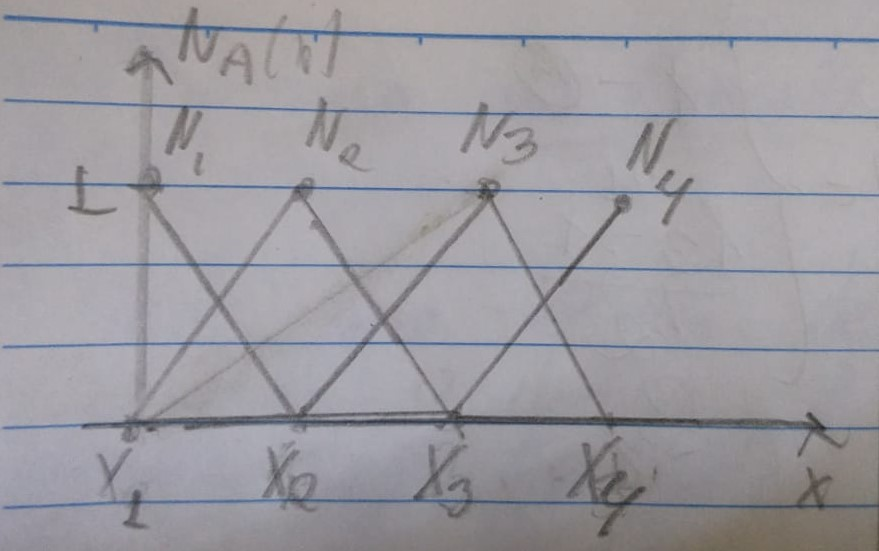
\includegraphics[scale=0.5]{AA03_Nax.jpeg}
\end{center}

Discretizamos o domínio $\Omega = \left[0, 1\right]$ em 4 nós com espaçamento uniforme:

\[
    x_1 = 0 \quad , \quad x_2 = \frac{1}{3} \quad , \quad x_3 = \frac{2}{3} \quad , \quad x_4 = 1
\]

Com esses nós e o desenho das funções de base, temos as expressões das funções de base como

\[
    N_1(x) = \begin{cases}
        1 - 3x, & 0 \leq x \leq \frac{1}{3} \\
        \noalign{\vskip9pt}
        0,      & \textrm{caso contrário}
    \end{cases}
    \quad , \quad
    N_2(x) = \begin{cases}
        3x,     & 0 \leq x \leq \frac{1}{3}           \\
        \noalign{\vskip9pt}
        2 - 3x, & \frac{1}{3} \leq x \leq \frac{2}{3} \\
        \noalign{\vskip9pt}
        0,      & \textrm{caso contrário}
    \end{cases}
\]

\[
    N_3(x) = \begin{cases}
        3x - 1, & \frac{1}{3} \leq x \leq \frac{2}{3} \\
        \noalign{\vskip9pt}
        3 - 3x, & \frac{2}{3} \leq x \leq 1           \\
        \noalign{\vskip9pt}
        0,      & \textrm{caso contrário}
    \end{cases}
    \quad , \quad
    N_4(x) = \begin{cases}
        3x - 2, & \frac{2}{3} \leq x \leq 1 \\
        \noalign{\vskip9pt}
        0,      & \textrm{caso contrário}
    \end{cases}
\]

Conhecidas as funções de base, agora precisamos encontrar as matrizes $K$, $d$ e $F$ do sistema matricial de \eqref{eqkdf}.
Sabemos que a matriz $K$ é $3 \times 3$ da forma

\begingroup
\renewcommand*{\arraystretch}{2}

\[
    K =
    \begin{bmatrix}
        K_{11} & K_{12} & K_{13} \\
        K_{21} & K_{22} & K_{23} \\
        K_{31} & K_{32} & K_{33}
    \end{bmatrix}
\]

\endgroup

Podemos usar duas propriedades da matriz de rigidez para reduzir a quantidade de contas que teremos que fazer.
\begin{itemize}
    \item A matriz é simétrica em relação à diagonal principal;
    \item A matriz é esparsa: elementos não vizinhos aos elementos da diagonal principal são nulos;
\end{itemize}

Assim, temos

\begingroup
\renewcommand*{\arraystretch}{2}

\[
    K =
    \begin{bmatrix}
        K_{11} & K_{12} & 0      \\
        K_{12} & K_{22} & K_{23} \\
        0      & K_{23} & K_{33}
    \end{bmatrix}
\]

\endgroup

Calculando os elementos um de cada vez, temos

\[
    K_{11} = a\left(N_1, N_1\right) = \int_{0}^{1} N_{1_x} N_{1_x} \, dx = \int_{0}^{\frac{1}{3}} (-3) (-3) \, dx = 3
\]

\[
    K_{12} = a\left(N_1, N_2\right) = \int_{0}^{1} N_{1_x} N_{2_x} \, dx = \int_{0}^{\frac{1}{3}} (-3) (3) \, dx = - 3
\]

\[
    K_{22} = a\left(N_2, N_2\right) = \int_{0}^{1} N_{2_x} N_{2_x} \, dx =
    \int_{0}^{\frac{1}{3}} (3) (3) \, dx + \int_{\frac{1}{3}}^{\frac{2}{3}} (-3) (-3) \, dx  = 6
\]

\[
    K_{23} = a\left(N_2, N_3\right) = \int_{0}^{1} N_{2_x} N_{3_x} \, dx =
    \int_{\frac{1}{3}}^{\frac{2}{3}} (-3) (3) \, dx  = -3
\]

\[
    K_{33} = a\left(N_3, N_3\right) = \int_{0}^{1} N_{3_x} N_{3_x} \, dx =
    \int_{\frac{1}{3}}^{\frac{2}{3}} (3) (3) \, dx + \int_{\frac{2}{3}}^{1} (-3) (-3) \, dx  = 6
\]

Assim, a matriz $K$ e sua inversa $K^{-1}$ são dadas por

\begingroup
\renewcommand*{\arraystretch}{2}

\[
    K =
    \begin{bmatrix}
        3  & -3 & 0  \\
        -3 & 6  & -3 \\
        0  & -3 & 6
    \end{bmatrix}
    \logo K^{-1} = \frac{1}{3}
    \begin{bmatrix}
        3 & 2 & 1 \\
        2 & 2 & 1 \\
        1 & 1 & 1
    \end{bmatrix}
\]

\endgroup

O próximo passo é calcular o vetor de forças $F$. Calculando um elemento de cada vez, temos

\[
    F_1 = (N_1, f) + N_1(0)h - a\left(N_1, qN_4\right) =
    \int_{0}^{1} \rho N_1(x) \, dx + (1)h - \int_{0}^{1} N_{1_x} qN_{4_x}
\]

\[
    = \rho \int_{0}^{\frac{1}{3}}  1 - 3x \, dx + h - 0 = \rho \left[x - 3\frac{x^2}{2}\right]_{0}^{\frac{1}{3}} + h
    = \rho \left(\frac{1}{3} - \frac{3}{2}\frac{1}{9}\right) + h = h + \frac{1}{6}\rho
\]

\[
    F_2 = (N_2, f) + N_2(0)h - a\left(N_2, qN_4\right) =
    \int_{0}^{1} \rho N_2(x) \, dx
\]

\[
    = \rho \left[\int_{0}^{\frac{1}{3}}  3x \, dx  + \int_{\frac{1}{3}}^{\frac{2}{3}}  2 - 3x \, dx\right] =
    \rho \left[\frac{3}{2}\frac{1}{9} + \left(2x - \frac{3}{2}x^2\right)_{\frac{1}{3}}^{\frac{2}{3}}  \right]
    = \rho \left(\frac{1}{6} + \frac{1}{6}\right) = \frac{1}{3}\rho
\]

\[
    F_3 = (N_3, f) + N_3(0)h - a\left(N_3, qN_4\right) =
    \int_{0}^{1} \rho N_3(x) \, dx - \int_{\frac{2}{3}}^{1} N_{3_x} qN_{4_x} \, dx
\]

\[
    = \rho \left[\int_{\frac{1}{3}}^{\frac{2}{3}}  3x - 1 \, dx  + \int_{\frac{2}{3}}^{1}  3 - 3x \, dx\right] - q\int_{\frac{2}{3}}^{1} (-3) (3) \, dx =
    \rho \frac{1}{3} + 3q
\]

Assim, temos o vetor de forças

\begingroup
\renewcommand*{\arraystretch}{2}

\[
    F =
    \begin{bmatrix}
        h + \frac{1}{6}\rho \\
        \frac{1}{3}\rho     \\
        \rho \frac{1}{3} + 3q
    \end{bmatrix}
\]

\endgroup

Finalmente, usando \eqref{eqdkf}, o sistema matricial que nos dá a solução do vetor de coeficientes $d$ é

\begingroup
\renewcommand*{\arraystretch}{2}

\[
    \begin{bmatrix}
        d_1 \\
        d_2 \\
        d_3
    \end{bmatrix} =
    \frac{1}{3}
    \begin{bmatrix}
        3 & 2 & 1 \\
        2 & 2 & 1 \\
        1 & 1 & 1
    \end{bmatrix}
    \begin{bmatrix}
        h + \frac{1}{6}\rho \\
        \frac{1}{3}\rho     \\
        \rho \frac{1}{3} + 3q
    \end{bmatrix}
\]

\endgroup

Substituindo os valores do enunciado do problema,

\begingroup
\renewcommand*{\arraystretch}{2}

\[
    \begin{bmatrix}
        d_1 \\
        d_2 \\
        d_3
    \end{bmatrix} =
    \frac{1}{3}
    \begin{bmatrix}
        3 & 2 & 1 \\
        2 & 2 & 1 \\
        1 & 1 & 1
    \end{bmatrix}
    \begin{bmatrix}
        \frac{11}{6} \\
        \frac{5}{3}  \\
        \frac{14}{3}
    \end{bmatrix}
    \logo
    \begin{bmatrix}
        d_1 \\
        d_2 \\
        d_3
    \end{bmatrix} =
    \begin{bmatrix}
        \frac{9}{2}  \\
        \frac{35}{9} \\
        \frac{49}{18}
    \end{bmatrix}
\]

\endgroup

Assim, a solução do problema encontrada pelo FEM é

\begin{equation}\label{eqUfem}
    \boxed{u^h(x) = \frac{9}{2}N_1(x) + \frac{35}{9}N_2(x) + \frac{49}{18}N_3(x) + N_{4}(x)}
\end{equation}

Plotando a solução obtida pelo FEM \eqref{eqUfem} e a solução analítica \eqref{eqUsubstituida} com o software online Desmos,
temos

\begin{center}
    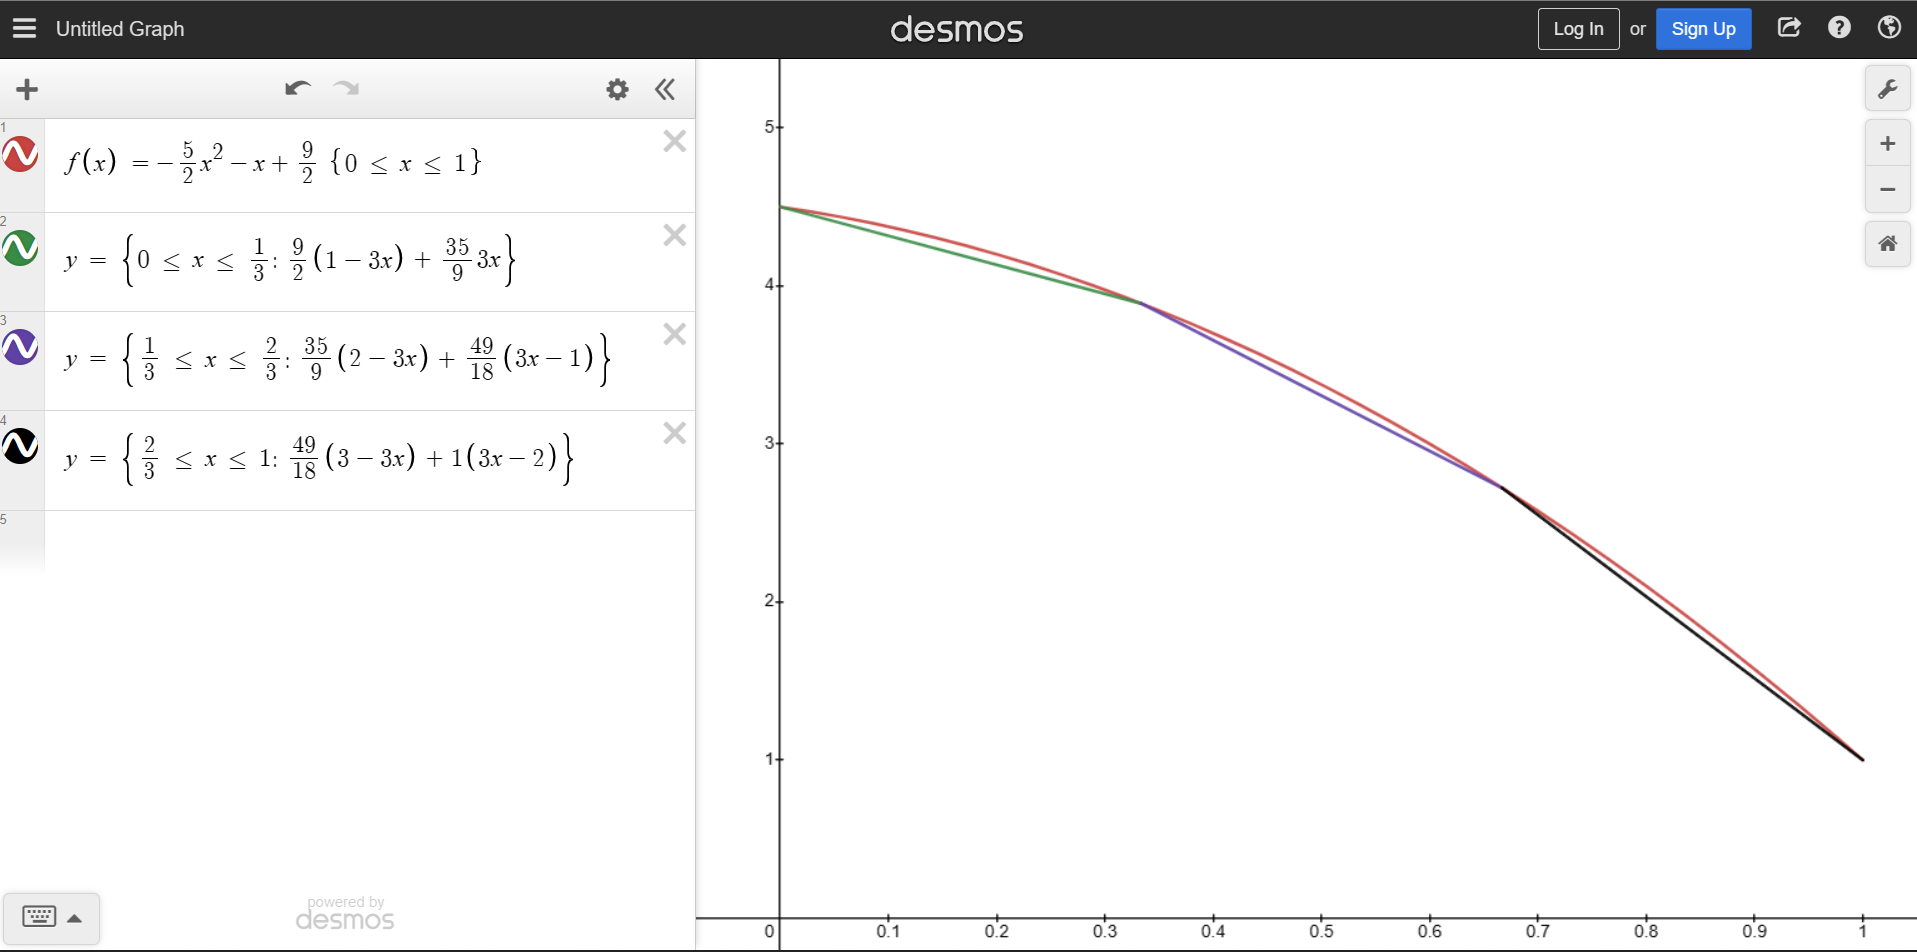
\includegraphics[scale=0.35]{grafico_ux_AA03.png}
\end{center}

\begin{center}
    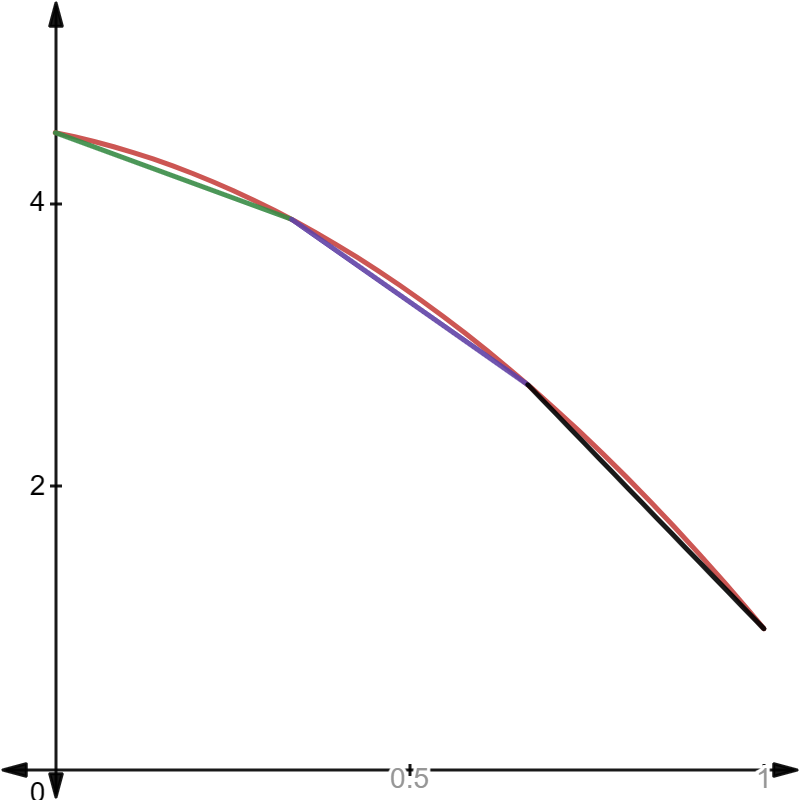
\includegraphics[scale=0.25]{grafico_zoom_ux_AA03.png}
\end{center}

A curva vermelha se refere à solução $u(x)$ analítica, e as demais retas são as soluções encontradas pelo FEM com três graus de liberdade.
É possível ver que, com apenas três graus de liberdade, o FEM se aproxima da solução analítica com bastante precisão e baixo erro.
Além disso, nos 4 nós selecionados, temos que a solução do FEM é igual à solução analítica.
\newline
Podemos fazer a mesma análise gráfica com as derivadas das soluções. A derivada $u_x$ da solução analítica é

\begin{equation}\label{eqDu}
    u_x(x) = -5x - 1
\end{equation}

A derivada da solução do FEM é

\begin{equation}\label{eqUfemD}
    u_x^h(x) = \frac{9}{2}N_{1_x}(x) + \frac{35}{9}N_{2_x}(x) + \frac{49}{18}N_{3_x}(x) + N_{4_x}(x)
\end{equation}

onde

\[
    N_{1_x}(x) = \begin{cases}
        -3, & 0 \leq x \leq \frac{1}{3} \\
        \noalign{\vskip9pt}
        0,      & \textrm{caso contrário}
    \end{cases}
    \quad , \quad
    N_{2_x}(x) = \begin{cases}
        3,     & 0 \leq x \leq \frac{1}{3}           \\
        \noalign{\vskip9pt}
        -3, & \frac{1}{3} \leq x \leq \frac{2}{3} \\
        \noalign{\vskip9pt}
        0,      & \textrm{caso contrário}
    \end{cases}
\]

\[
    N_{3_x}(x) = \begin{cases}
        3, & \frac{1}{3} \leq x \leq \frac{2}{3} \\
        \noalign{\vskip9pt}
        -3, & \frac{2}{3} \leq x \leq 1           \\
        \noalign{\vskip9pt}
        0,      & \textrm{caso contrário}
    \end{cases}
    \quad , \quad
    N_{4_x}(x) = \begin{cases}
        3, & \frac{2}{3} \leq x \leq 1 \\
        \noalign{\vskip9pt}
        0,      & \textrm{caso contrário}
    \end{cases}
\]

Assim, plotando \eqref{eqDu} e \eqref{eqUfemD} no Desmos, temos

\begin{center}
    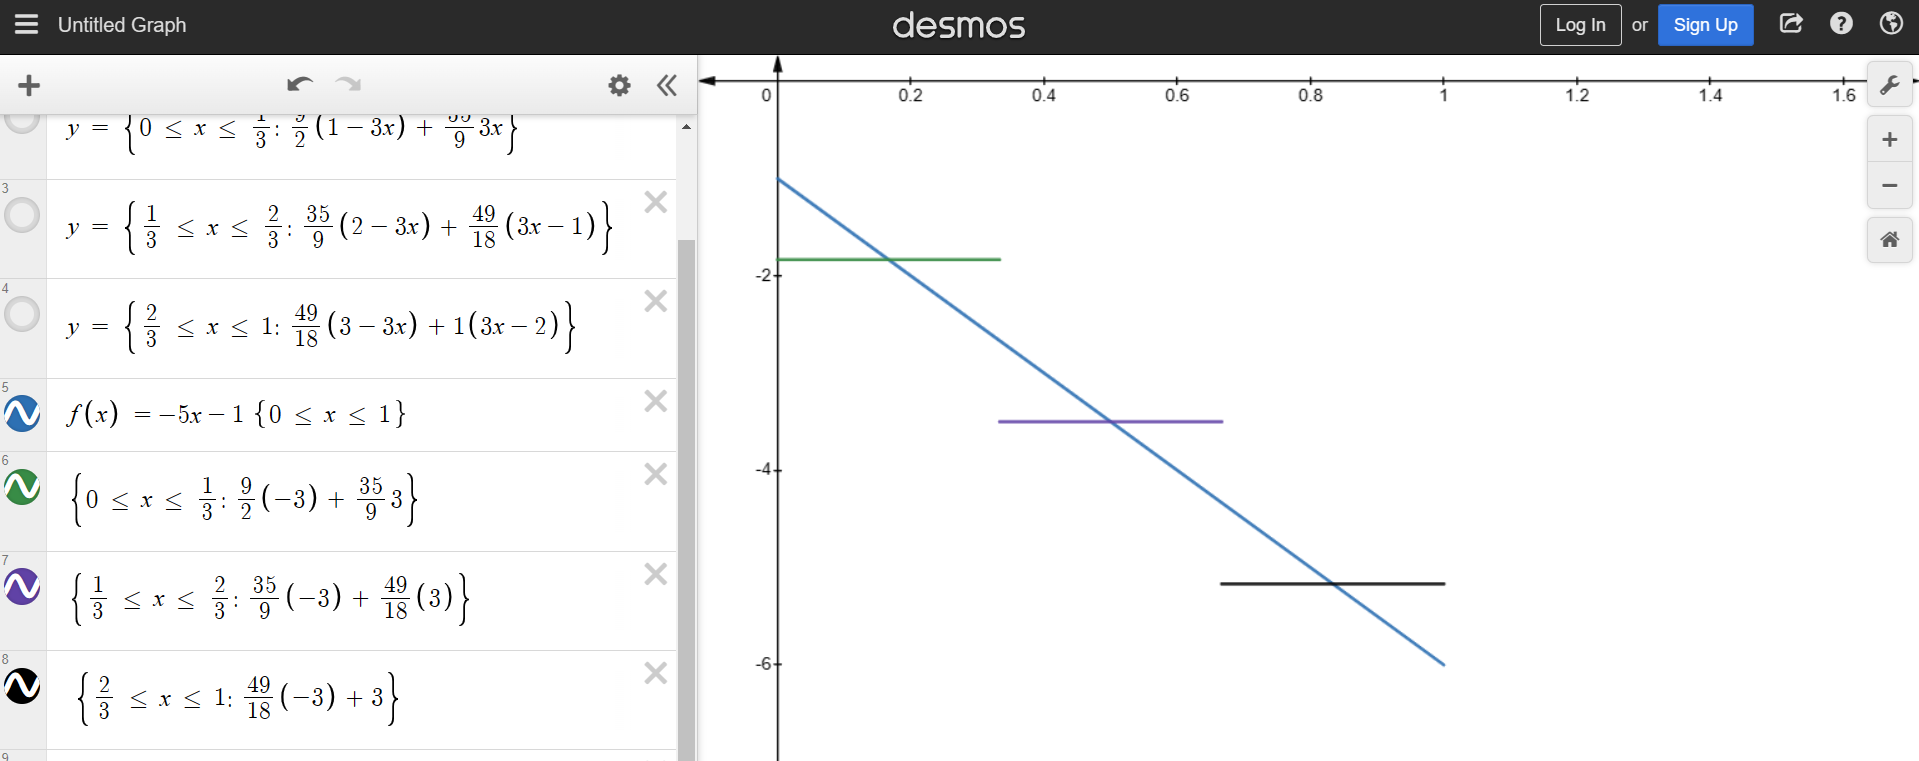
\includegraphics[scale=0.35]{grafico_dudx_AA03.png}
\end{center}

Vemos que a derivada da solução analítica (curva azul) é igual à derivada da solução do FEM (demais curvas da imagem) em 
apenas em três pontos, que corresponde aos três graus de liberdades adotado na aplicação do método.

\end{document}



